% 请将代码块设置为按缩进,方便区分功能块
% 本模版旨在让你像使用 Word 一样使用 LaTeX


%--------------------------文档格式---------------------------%
	\documentclass[10pt,a4paper,column,twoside,UTF8]{ctexart}
		% 10pt:设置正文字体大小,但各层级字体大小会根据正文字体自动调整
		% twocolumn:双栏排版;
		% twoside:分奇偶页;
%-----------------------------------------------------------%


%-------------------------页边距设置--------------------------%
	\usepackage{geometry}
		% 用于设置上下左右页边距
		\geometry{left=1cm,right=1cm,top=2.5cm,bottom=4cm}
		% 设置两栏目之间的间距
		\setlength\columnsep{0.85cm}
%-----------------------------------------------------------%


%--------------------------各种宏包---------------------------%
	\usepackage{xeCJK,amsmath,paralist,enumerate,booktabs,multirow,graphicx,float,subfig,setspace}
		% xeCJK:中文字体的设置
		% amsmath:数学公式
		% graphicx,float: 插入图片
		% setspace:设置行间距等功能
		\setlength{\parindent}{2em}		
		% 正文首行缩进两个汉字

	\setCJKmainfont{FZShuSong-Z01S}[ItalicFont=FZKai-Z03S, BoldFont=FZHei-B01S]
	% 中文字体设置:使用开源字体方正书宋,方正楷体和方正黑体

	\usepackage{titlesec}
	% 改变section、subsection里面字体的样式。中文黑体,英文TNR。
		\newfontfamily\sectionef{Times New Roman}
		\setCJKfamilyfont{FZHeiTi}{FZHei-B01S}
		\newcommand{\sectioncf}{\CJKfamily{FZHeiTi}}
		\titleformat*{\section}{\large\bfseries\sectioncf\sectionef}
		\titleformat*{\subsection}{\normalsize\bfseries\sectioncf\sectionef}


	\usepackage{fancyhdr}
	%fancyhdr:一个很强大的宏包,用于自定义设计页面风格并命名以供调用。

	\usepackage{gbt7714}
	% 使用gbt7714的Bibtex参考文献风格
%-----------------------------------------------------------%


%-----------------------代码块风格设置-------------------------%
	\usepackage{xcolor,listings}
		\lstset
		{	language=Matlab,	% 代码类型MATLAB
			breaklines,			% 自动换行
			columns=flexible,	% 不自动添加空格
			frame=l,			% 背景框
			numbers=left,		% 行号的设定
			numberstyle=\tiny\color{gray},
			basicstyle=\small\ttfamily,							% 基本样式
			backgroundcolor=\color[RGB]{245,245,244},			% 设定背景颜色
			keywordstyle=\color[RGB]{40,40,255},                % 设定关键字颜色
			commentstyle=\it\color[RGB]{0,96,96},               % 设置代码注释的格式
			stringstyle=\ttfamily\slshape\color[RGB]{128,0,0},	% 设置字符串的格式
		}
%-----------------------------------------------------------%


%-------------------设置首页和正文不同的页眉页脚-----------------%

	\usepackage{ifthen}%这个宏包提供逻辑判断命令
	\newboolean{first}%引入布尔变量
	\setboolean{first}{true}%将布尔变量设置为true
	\pagestyle{fancy}

		%%% Step1 定义正文的页面风格
		% E表示偶数页,O表示奇数页;R、L、C代表文字居右、居左、居中排版
		% 页码:保证在外侧, 奇数页分布在右边,偶数页分布在左边
		% 页眉中间的内容也因奇偶页而不同
		% 实验名称根据实际情况修改
		\fancypagestyle{maincontent}{
			\fancyhf{}  	% 清空页眉页脚设置
			\fancyhead[EL, OR]{\thepage}
			\fancyhead[EC]{可替换文字一}
			\fancyhead[OC]{可替换文字二}
			\renewcommand\headrulewidth{0pt}
		}

		%%% Step2 定义首页的页面风格
		% 页眉中间的双行文字,大小和字间距需要微调
		% 左右的内容是年月,可以自己修改寻找自动获取的方法
		\usepackage{datetime}
		\fancypagestyle{firstpage}{
			\setboolean{first}{false} 	% firstpage出现,则将first重置为false
			\fancyhf{}  				% 清空页眉页脚设置
			\fancyhead[L]{\the\year 年\the\month 月}
			\fancyhead[R]{\shortmonthname[\the\month], \the\year}
			\fancyhead[C]{
					\large{可替换文字二}\\
					\small{Optional English Name}
					}
		}

		%%% Step3 页眉线的设置:用布尔变量区分首页和正文
		\newcommand{\makefirstpageheadrule}{								% 定义首页页眉线-双线绘制命令
			\makebox[0pt][l]{\rule[0.55\baselineskip]{\headwidth}{0.2pt}}	% 上0.5pt,下0.2pt
			\rule[0.7\baselineskip]{\headwidth}{0.5pt}
		}

		\newcommand{\makeheadrule}{											% 定义正文页页眉线绘制命令,单线
			\rule[0.7\baselineskip]{\headwidth}{0.75pt}
		}

		% 根据布尔变量first为true或false分别执行不同的页眉线绘制命令
		\renewcommand{\headrule}{											% 重定义headrule命令
			\ifthenelse{\boolean{first}}{\makeheadrule}
			{\makefirstpageheadrule}
		}
%-----------------------------------------------------------%


\begin{document}	% 文档从此处开始


%-------------------------摘要------------------------------%


	\title{\LARGE\textbf{可替换文字一}}
	\author{\large\textit{您的姓名}$^{1}$\\ \normalsize{(1 \textit{您的大学,您的学院,某省~某市}~000000)}}
	\date{}	% 不显示日期

	\twocolumn[
		% twocolumn: 双栏article下的单栏摘要
		\begin{@twocolumnfalse}
		\maketitle  					% 标题和作者
		\renewcommand{\abstractname} {} % 不显示摘要名字
		\begin{abstract}
		\vspace{-3em}
		% vspace:调整垂直空白,可以自己调整;缩小abstract和center(以及maketitle)的间距
		% \noindent 摘要无缩进
		\textbf{摘 要:}
		{\small 摘要}
		\par
		\textbf{关键词:}关键词;分号;隔开
		\vspace{2em}
		\end{abstract}
		\end{@twocolumnfalse}
	]

	\thispagestyle{firstpage}	% 首页页面风格:firstpage
	\pagestyle{maincontent}		% 第二页之后的页面风格:maincontent
%-----------------------------------------------------------%




%-------------------------正文------------------------------%
	\section{实验原理}
		关于浦丰投针实验的叙述如下:假设有以平行且等距的木纹铺成的
		地板,现在随意抛一支长度比木纹之间距离小的针,求针和其中一条木纹相交的概率。
		\par
		为了方便进行模拟实验,
		我们将该情景抽象成数学模型,并转述如下:\emph{假设有间距为a的无限细长平行线,
		随机地将长度固定为l的线段放置在平行线之间,求针和平行线相交的概率。}
		\par
		对于该实验普遍的方法是,我们可以通过研究针中点到最近平行线的距离$x$
		和针与平行线形成的上方夹角 $\alpha$ 来判断相交情况,如图所示:

		\begin{figure}[htbp]
			\centering
			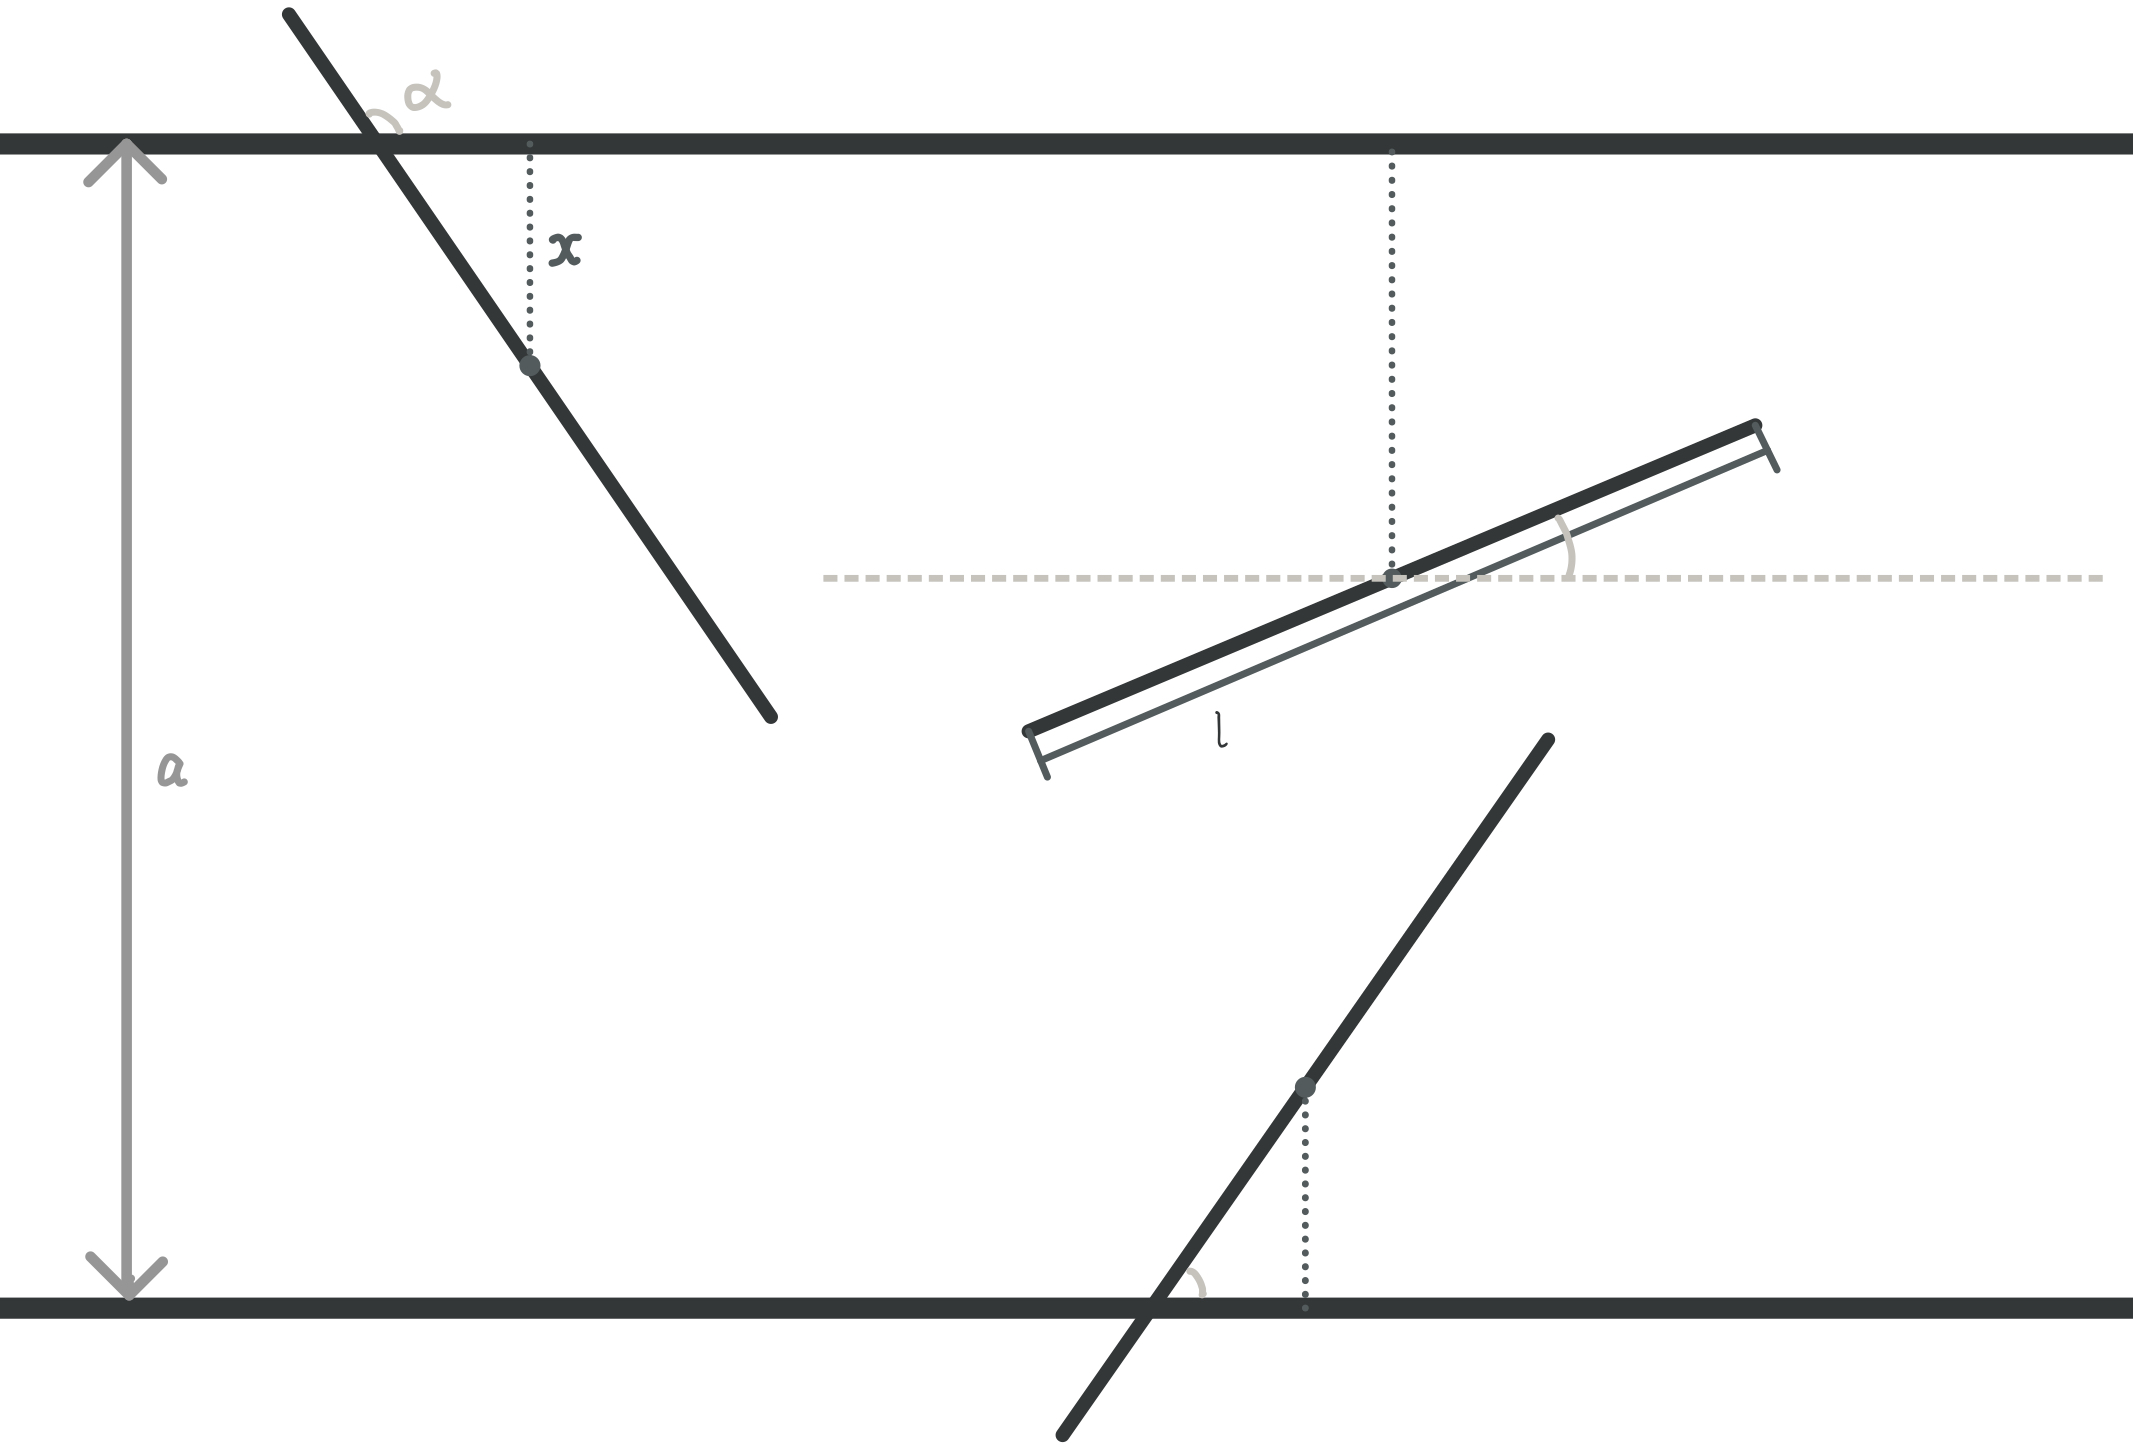
\includegraphics[width=0.4\textwidth]{illustration0.jpeg}
				%textwidth:正文宽度。双栏,则将两栏正文宽度相加。
			\caption{投针模型演示}
		\end{figure}
		当针和平行线相交时,$x$和$\alpha$应满足如下不等式
		\begin{equation}
			x \leq \frac{l}{2}sin\alpha
		\end{equation}

		同时,这由于$x$是中点到\emph{最近}平行线的距离,
		而$\alpha$是上方夹角,所以两个变量应满足
		\begin{gather}
			0 \leq x \leq \frac{a}{2}\\
			0 \leq \alpha \leq \pi
		\end{gather}

	% section后面的正文:自动换段,正常缩进
	% 自然换段:\par
	% \newpage
	% 换一栏,而不是换一页。换一页用\clearpage

	\section{MATLAB模拟}
		% 文献引用已启用
		这句话不是我说的,是小明\cite{example}说的。
%-----------------------------------------------------------%




%------------------------参考文献----------------------------%
	% 使用
	\bibliographystyle{gbt7714-numerical}
	\bibliography{reference.bib}
%-----------------------------------------------------------%


\end{document}		% 文档在此处结束

